% !TeX root = ../slides.tex
% 09-results.tex — headline experiment, real wandb/checkpoint results.

\section{Results}

\begin{frame}{Experimental Setup}
  \begin{itemize}
    \item board: $6 \times 6$, $5$ mines (density $\approx 13.9\%$),
      \alert{identical} for DQN and PPO;
    \item $150{,}000$ training episodes for both agents;
    \item disjoint RNG seed ranges for train / validation / held-out test
      (no leakage between phases);
    \item periodic validation rollouts (masked, greedy) select the
      \alert{best} checkpoint by win rate, saved alongside its
      \texttt{wandb\_run\_id};
    \item final evaluation: $1{,}000$ held-out test episodes per agent,
      run via \texttt{main.py test} on the selected checkpoint.
  \end{itemize}
\end{frame}

\begin{frame}{Training Curves — 150k Episodes}
  \centering
  \begin{columns}[T, totalwidth=\textwidth]
    \begin{column}{0.48\textwidth}
      \centering
      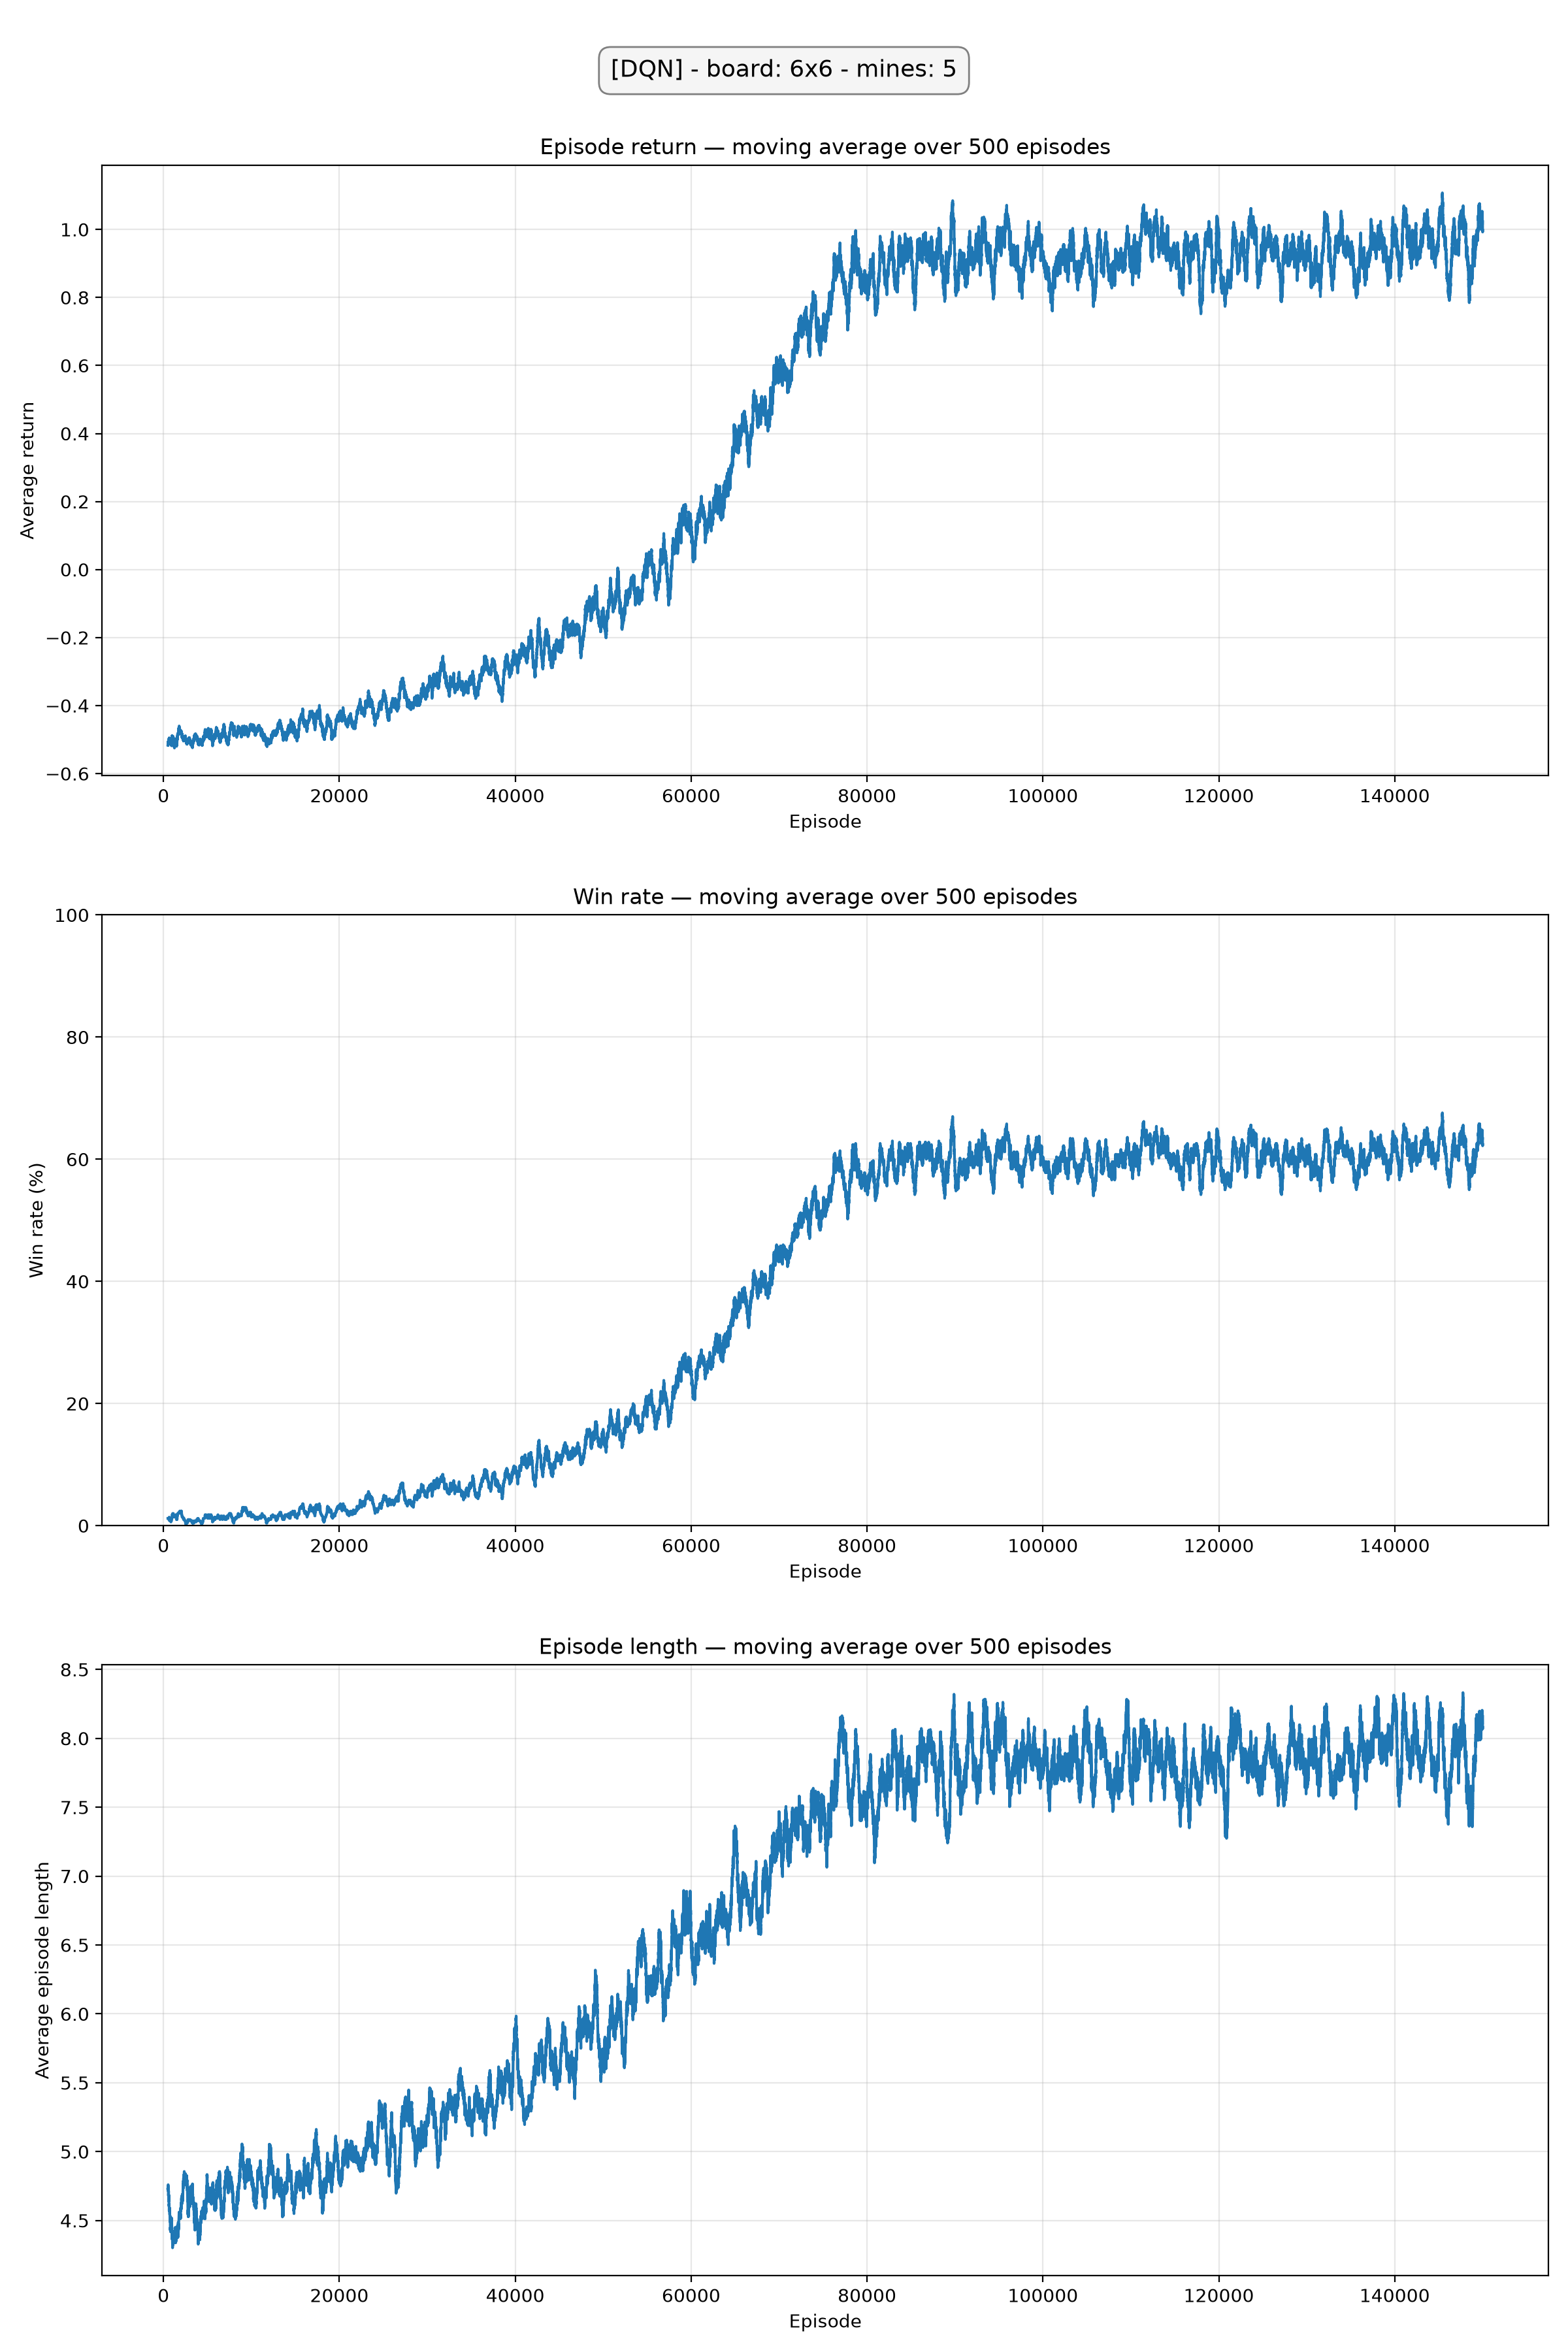
\includegraphics[height=5.8cm]{assets/results/dqn_training_curves.png}\\
      \small \textbf{DQN}
    \end{column}
    \begin{column}{0.48\textwidth}
      \centering
      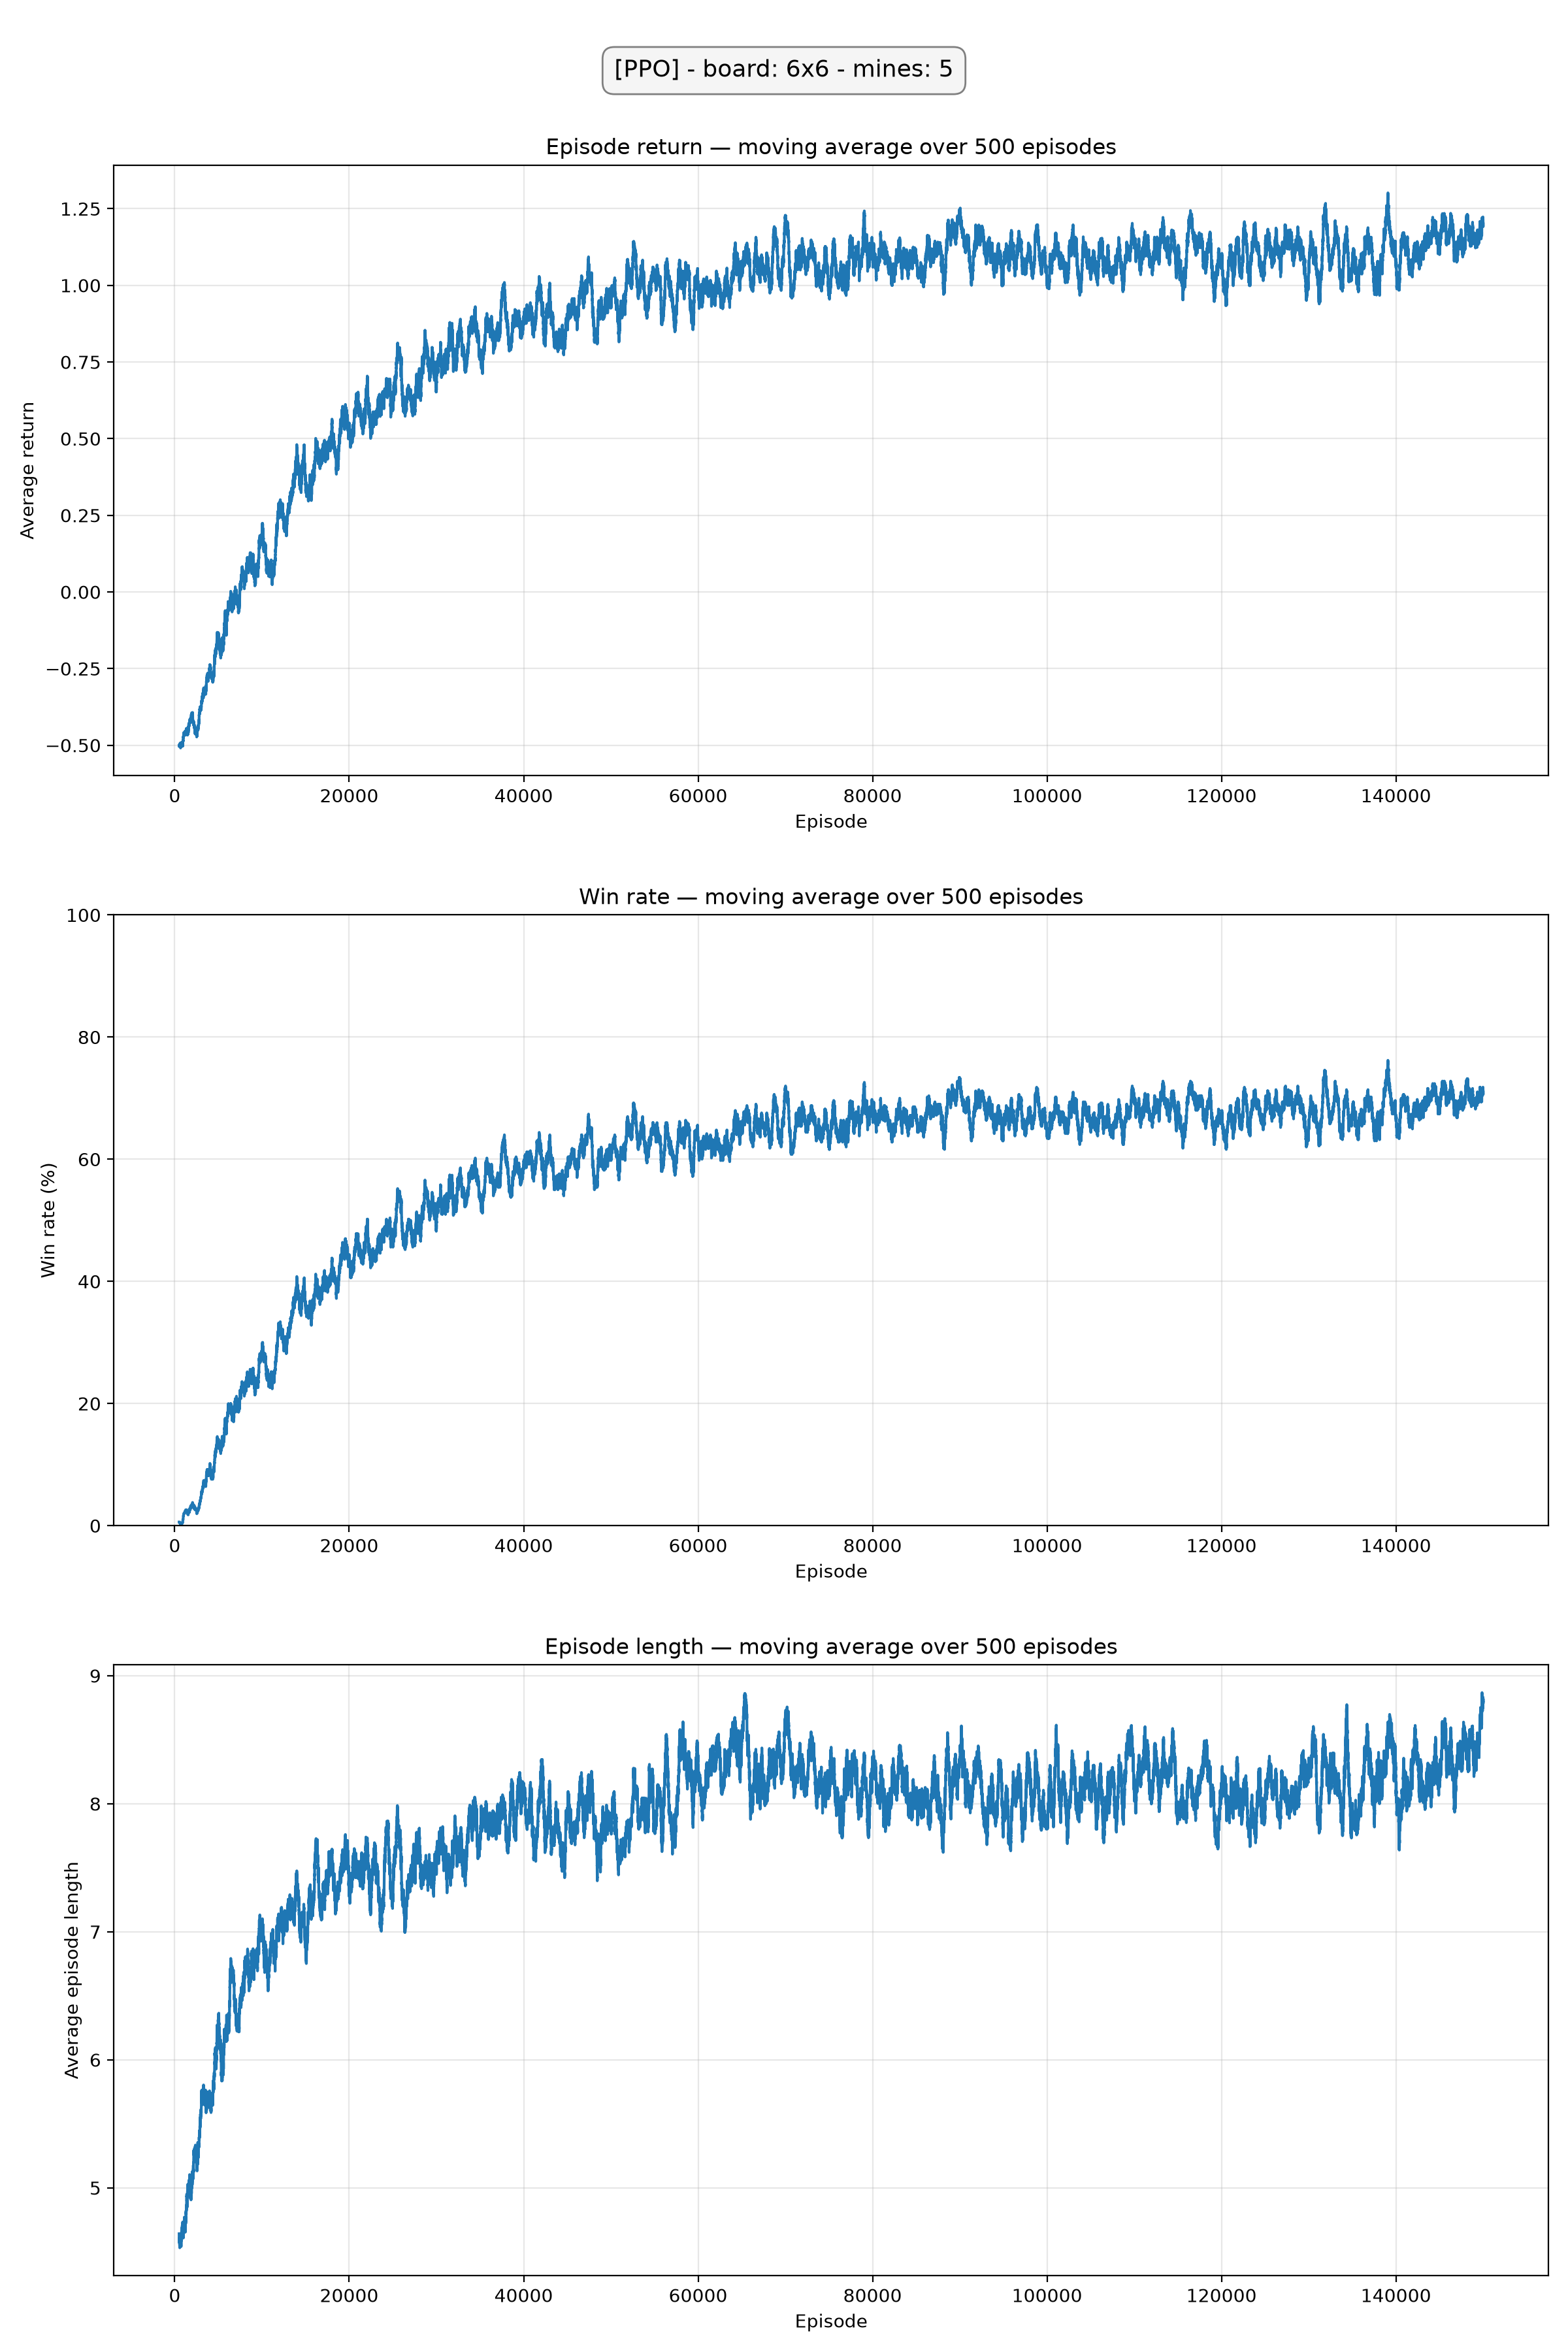
\includegraphics[height=5.8cm]{assets/results/ppo_training_curves.png}\\
      \small \textbf{PPO}
    \end{column}
  \end{columns}
  {\tiny return, win rate, episode length — 500-episode moving average}
\end{frame}

\begin{frame}{Held-Out Test Reports (1000 episodes)}
  \centering
  \begin{columns}[T, totalwidth=\textwidth]
    \begin{column}{0.48\textwidth}
      \centering
      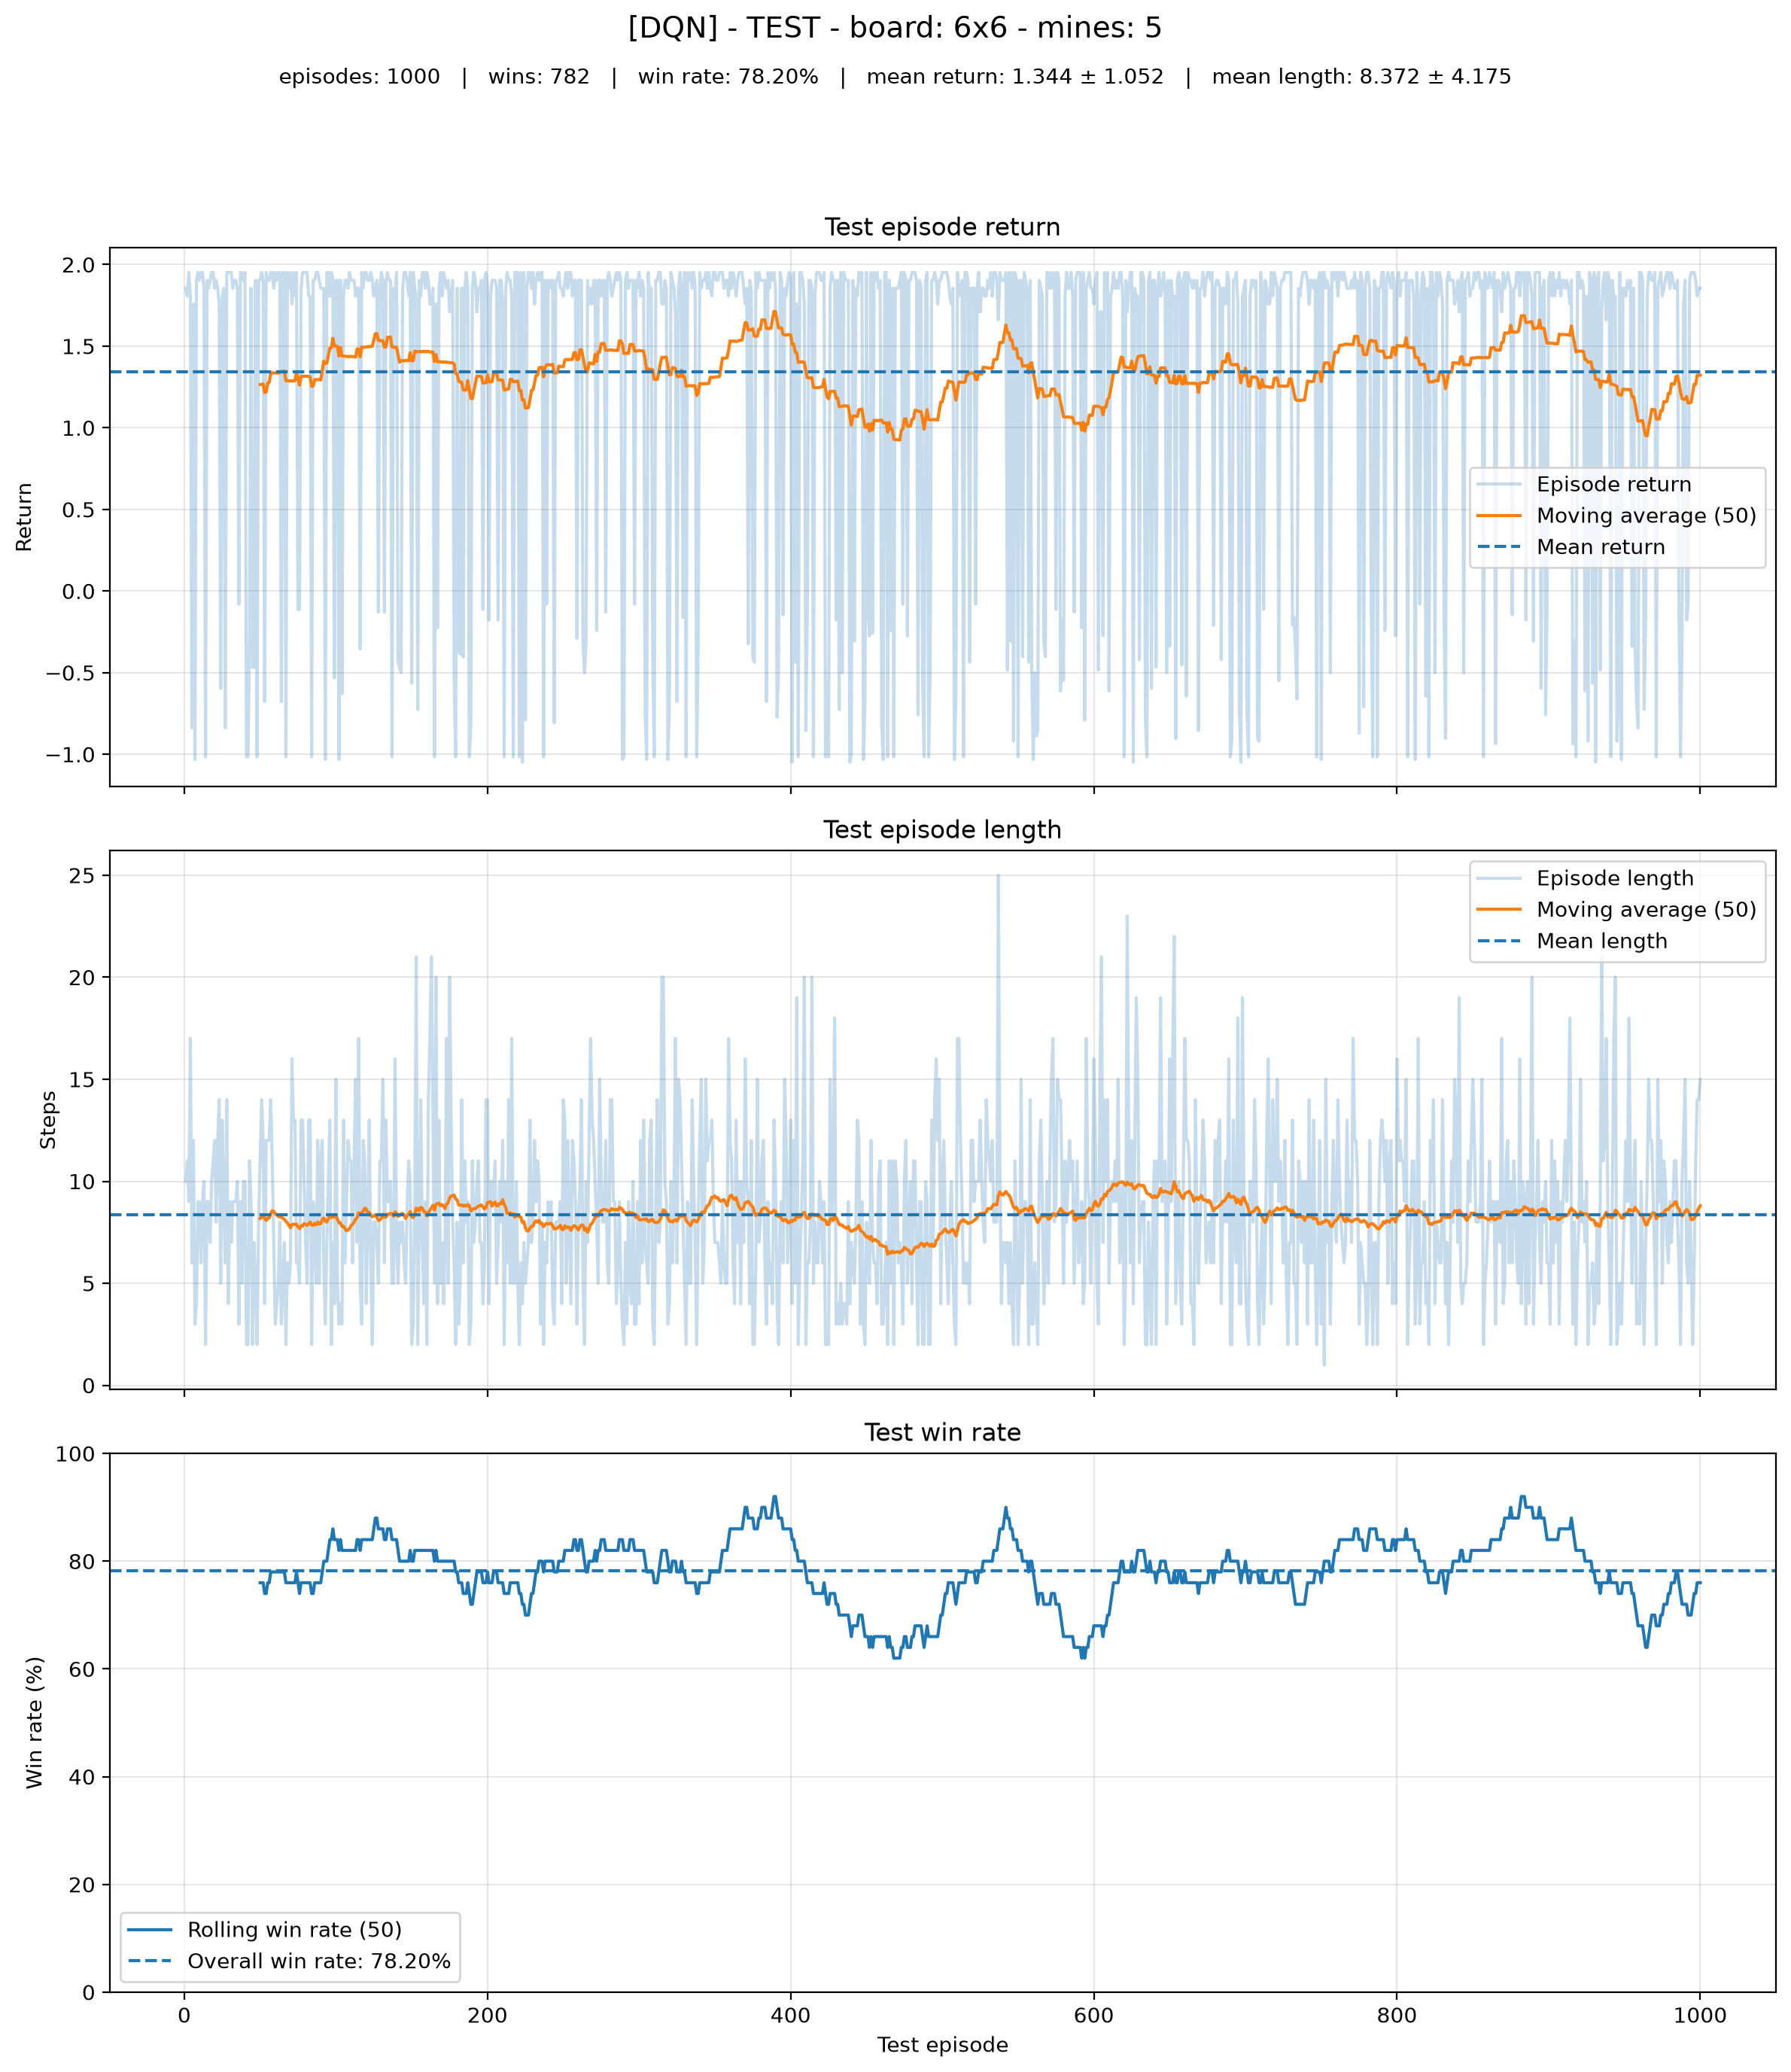
\includegraphics[height=5.6cm]{assets/results/dqn_test_report.png}\\
      \small \textbf{DQN} — 782/1000 wins
    \end{column}
    \begin{column}{0.48\textwidth}
      \centering
      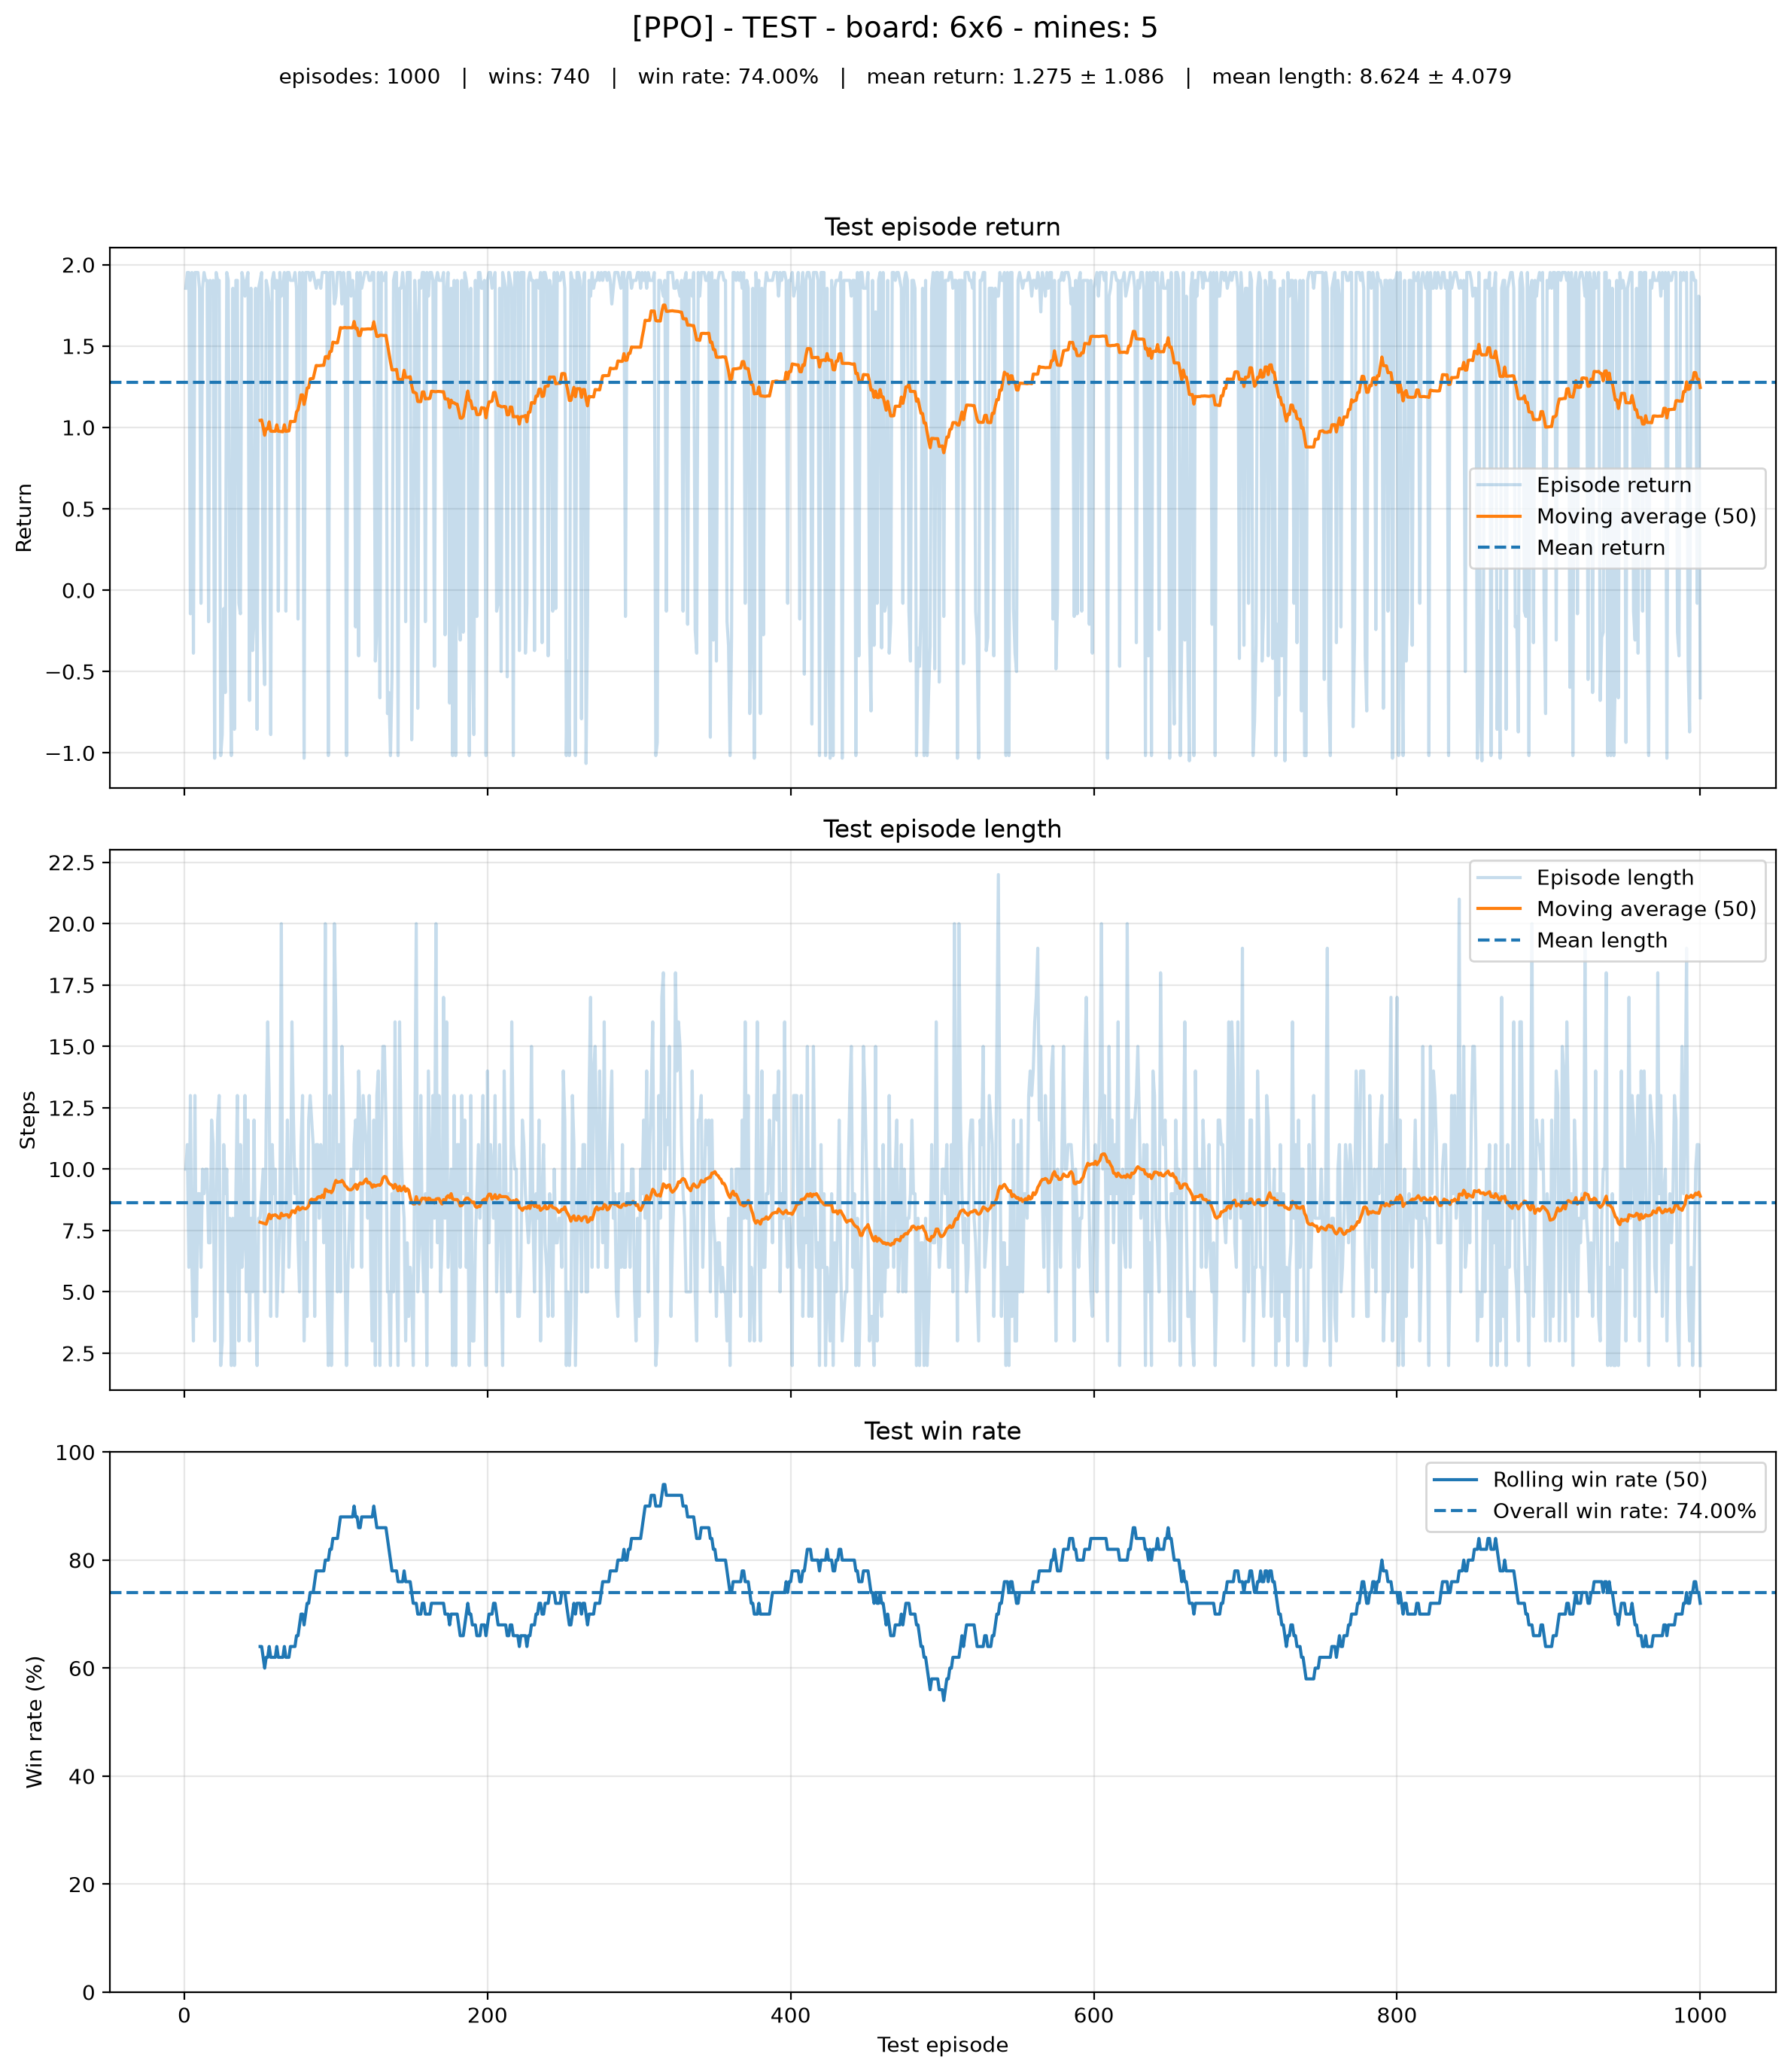
\includegraphics[height=5.6cm]{assets/results/ppo_test_report.png}\\
      \small \textbf{PPO} — 740/1000 wins
    \end{column}
  \end{columns}
\end{frame}

\begin{frame}{DQN vs PPO — Head to Head}
  \begin{figure}
    \centering
    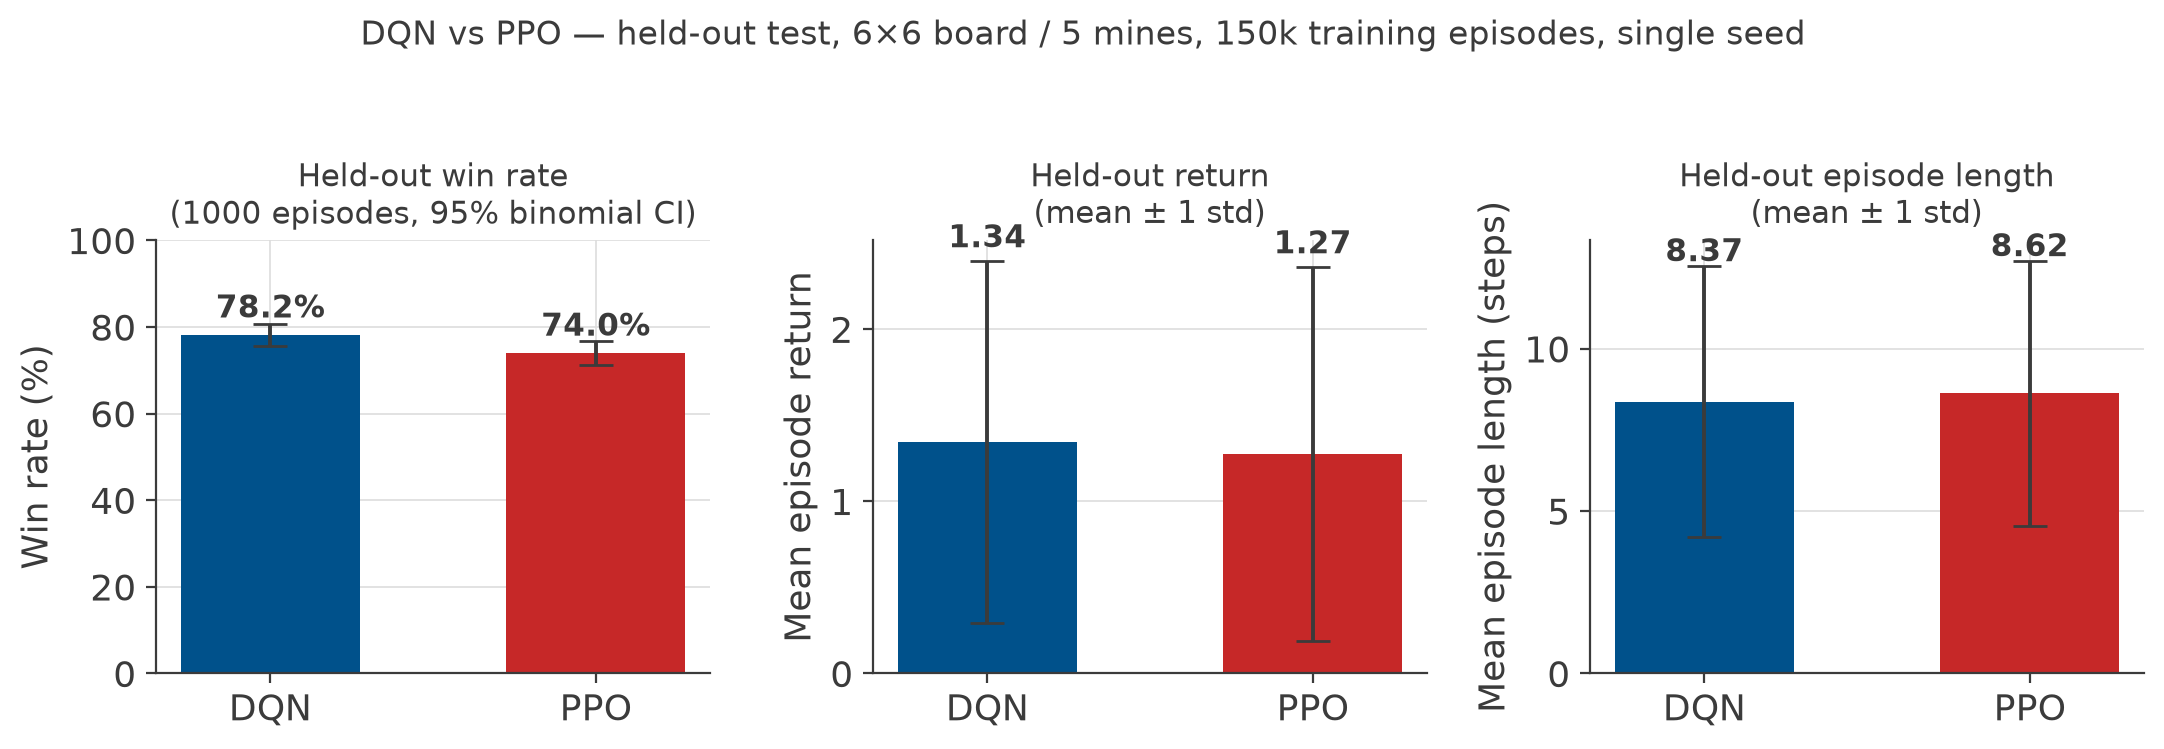
\includegraphics[width=0.85\textwidth]{assets/results/dqn_ppo_comparison.png}
  \end{figure}
  {\scriptsize\noindent Win-rate error bars are 95\% binomial CIs ($n=1000$); return/length error bars are $\pm 1$ std over the 1000 test episodes.\par}
  \vspace{0.15cm}
  \begin{center}
  \small
  \renewcommand{\arraystretch}{0.9}
  \begin{tabular}{lccc}
    \toprule
    & \textbf{Win rate} & \textbf{Mean return} & \textbf{Mean length} \\
    \midrule
    DQN & $78.20\%$ & $1.344 \pm 1.052$ & $8.372 \pm 4.175$ \\
    PPO & $74.00\%$ & $1.275 \pm 1.086$ & $8.624 \pm 4.079$ \\
    \bottomrule
  \end{tabular}
  \end{center}
\end{frame}

\begin{frame}{Limitations \& Next Steps}
  \begin{itemize}
    \item \alert{single seed}: the $78.2\%$ vs $74.0\%$ gap is suggestive
      but the two binomial CIs are close — a rigorous comparison needs
      several training seeds per algorithm and a paired statistical test,
      as required by the SRLP guidelines;
    \item results are reported on \alert{one} fixed board configuration
      ($6\times6$/5 mines) — no evidence yet on generalization to larger
      boards or different mine densities, despite the board-size-agnostic
      architecture;
    \item no ablation isolating the contribution of the mine-density
      channel, of flood-fill reward shaping, or of action masking;
    \item DQN here uses uniform replay — no prioritized experience replay
      (\per{}) or distributional value estimation (\ddqn{}), both natural
      next steps given the existing macros already reserved for them.
  \end{itemize}
\end{frame}
